\chapter{Implementacija i korisničko sučelje}
		
		
		\section{Korištene tehnologije i alati}
		
			 Tijekom rada na projektu najveći dio komunikacije ostvaren je redovnim sastancima putem aplikacije \textit{Microsoft Teams}\footnote{https://www.microsoft.com/hr-hr/microsoft-365/microsoft-teams/}, aplikaciji namijenjenoj za komunikaciju članova tima. Za olakšan timski rad na projektu veliku zaslugu imao je i \textit{Git}\footnote{https://git-scm.com/}, alat za verzioniranje inačica i praćenje promjena, a kao udaljena platforma koristio se \textit{Gitlab}\footnote{https://gitlab.com/}.\newline
			  Kao razvojno okruženje koristio se \textit{IntellijIDEA} \footnote{https://www.jetbrains.com/idea}, a predstavlja integrirano razvojno okruženje napisano u Javi za razvoj računalnog softvera. Tehnologija na poslužiteljskoj strani bio je \textit{Spring Boot}\footnote{https://spring.io/projects/spring-boot}, radni okvir otvorenog koda korišten za stvaranje mikroservisa, a kod na poslužiteljskoj strani pisan je u programskom jeziku \textit{Java 11}. \textit{Spring Boot} je odabran zato što nudi veliku količinu gotovih funkcionalnosti visoke razine apstrakcije. Uz njega koristimo i poznatu knjižnicu \textit{Spring JPA}\footnote{https://spring.io/projects/spring-data-jpa} te ORM bibiloteku \textit{Hibernate}\footnote{https://hibernate.org/} koja služi za mapiranje objektno orijentiranog modela domena u relacijsku bazu podataka. Za vrijeme razvoja aplikacije korištena je privremena baza podataka \textit{H2}\footnote{https://www.h2database.com/}, a ona predstavlja neperzistentnu bazu podataka napisanu u programskom jeziku \textit{Java}. Kao produkcijska baza korištena je relacijska perzistentna baza podataka \textit{PostgreSQL}\footnote{https://www.postgresql.org/}, koja je besplatna i otvorenog koda, u \textit{Springu} dobro podržana. Kao alat za praćenje promjena, tzv. migracija baze podataka korišten je \textit{Liquibase} \footnote{https://www.liquibase.org/}. Za testiranje poslužiteljske strane korištena je knjižnica \textit{JUnit}\footnote{https://junit.org/junit5/}, namijenjena za testiranje komponenti.
			  \\Što se tiče klijentske strane korišten je \textit{React}\footnote{https://reactjs.org/}, a predstavlja \textit{Javascript}\footnote{https://www.javascript.com/} knjižnicu za izgradnju korisničkog sučelja ili UI komponenti. Kod na klijentskoj strani pisan je u programskom jeziku \textit{Typescript}\footnote{https://www.typescriptlang.org/}, a to je programski jezik koji je razvio \textit{Microsoft}, te u klasični \textit{Javascript} dodaje navođenje tipova podataka. Prilikom izvršavanja, prevodi se u \textit{Javascript} te se izvodi unutar preglednika. Osim toga korišten je standardni \textit{CSS} i \textit{HTML}, a neke gotove komponente preuzete su iz knjižnice gotovih \textit{React} komponenti, \textit{Material-UI}\footnote{https://material-ui.com/} te \textit{Semantic UI}\footnote{https://semantic-ui.com/}.\\
			  Za pisanje dokumentacije korišten je \textit{LaTeX}\footnote{https://www.latex-project.org/}, jezik za pisanje strukturiranih tekstova, a pisan unutar integracijskog radnog okruženja za pisanje \textit{LaTeX} dokumenata \textit{TexStudio}\footnote{https://www.texstudio.org/}. Svi potrebni dijagrami modelirani su pomoću alata \textit{Astah}\footnote{https://astah.net/}.
			 		
			\eject 
		
	
		\section{Ispitivanje programskog rješenja}
			
			\subsection{Ispitivanje komponenti}
			U 7 testova proveli smo ispitivanje sloja nadglednika za pretraživanje domova i stvaranje novog planinarskog doma od strane administratora, te 4 testa za pretragu planinarskih domova na servisnom sloju. Kako bismo testirali servisni sloj, napravili smo \textit{SQL} skriptu koja nam bazu podataka puni testnim podacima. Navedena skripta će biti prikazana prije navođena testova servisnog sloja.
			Za testiranje sloja nadglednika koristili smo \textit{MockMvc}, odnosno nema stvarne komunikacije s bazom podataka prilikom testiranja sloja nadglednika. Prilikom testiranja neke pomoćne metode nisu navede zbog prevelikog prostora koji zauzima cijeli kod.\\
			
			\subsubsection{Testiranje sloja nadglednika}
			
			\textbf{\textit{Ispitni slučaj 1: Pretraga planinarskih domova kada su sva polja null vrijednosti.}}\\
			Očekivani rezultat ovog testa je povratak svih domova koji se nalaze u bazi podataka, to je podrazumijevano pretraživanje domova.\\
			
			
			\begin{lstlisting}
				@Test
				public void GivenRequestAllFieldsNull_When_MountainLodgeSearch_Should_ReturnAllResults()
				throws Exception {
					
					List<MountainLodge> mountainLodges = MountainLodgeGeneratingUtil
					.generateLodgesEmptyUtilitiesAndImageNull(3);
					given(mountainLodgeQueryService
					.findAllMountainLodgeBySearchCriteria(any()))
					.willReturn(mountainLodges);
					
					mvc.perform(post("/mountain-lodges/search")
					.content("{}")
					.contentType(MediaType.APPLICATION_JSON))
					.andExpect(status().isOk())
					.andExpect(jsonPath("$", hasSize(3)))
					.andExpect(jsonPath("$[0].hillName", is("hill1")))
					.andExpect(jsonPath("$[1].hillName", is("hill2")))
					.andExpect(jsonPath("$[2].hillName", is("hill3")))
					.andExpect(jsonPath("$[0].name", is("lodge1")))
					.andExpect(jsonPath("$[1].name", is("lodge2")))
					.andExpect(jsonPath("$[2].name", is("lodge3")))
					.andExpect(jsonPath("$[0].id", is(1)))
					.andExpect(jsonPath("$[1].id", is(2)))
					.andExpect(jsonPath("$[2].id", is(3)));
					}
			\end{lstlisting}


			\textbf{\textit{Ispitni slučaj 2: Pretraga planinarskih domova, polje za pretragu sadrži prazan znakovni niz.}}\\
			Očekivani rezultat ovog testa je povratak svih domova koji se nalaze u bazi podataka.\\
			
			
			\begin{lstlisting}
				@Test
				public void GivenRequestSearchTextEmpty_When_MountainLodgeSearch_Should_ReturnAllResults()
				throws Exception {
					
					List<MountainLodge> mountainLodges = MountainLodgeGeneratingUtil
					.generateLodgesEmptyUtilitiesAndImageNull(3);
					given(mountainLodgeQueryService
					.findAllMountainLodgeBySearchCriteria(any())).willReturn(mountainLodges);
					
					mvc.perform(post("/mountain-lodges/search")
					.content("{\"searchText\":\"\"}")
					.contentType(MediaType.APPLICATION_JSON))
					.andExpect(status().isOk())
					.andExpect(jsonPath("$", hasSize(3)))
					.andExpect(jsonPath("$[0].hillName", is("hill1")))
					.andExpect(jsonPath("$[1].hillName", is("hill2")))
					.andExpect(jsonPath("$[2].hillName", is("hill3")))
					.andExpect(jsonPath("$[0].name", is("lodge1")))
					.andExpect(jsonPath("$[1].name", is("lodge2")))
					.andExpect(jsonPath("$[2].name", is("lodge3")))
					.andExpect(jsonPath("$[0].id", is(1)))
					.andExpect(jsonPath("$[1].id", is(2)))
					.andExpect(jsonPath("$[2].id", is(3)));
				}
		\end{lstlisting}
			\textbf{\textit{Ispitni slučaj 3: Pretraga planinarskih domova, sva polja sadržavaju dozvoljene vrijednosti.}}\\
			Očekivani rezultat ovog testa je povratak prazne liste domova, jer dom koji zadovoljava parametre ne postoji.\\
			
			
			\begin{lstlisting}
				@Test
				public void GivenRequestWithAllFields_When_MountainLodgeSearch_Should_ReturnEmptyList()
				throws Exception {
					
					List<MountainLodge> mountainLodges = Collections.emptyList();
					given(mountainLodgeQueryService
					.findAllMountainLodgeBySearchCriteria(any()))
					.willReturn(mountainLodges);
					
					mvc.perform(post("/mountain-lodges/search")
					.content(
					"{\"searchText\":\"planinarski dom graficar\",
						\"hillId\":\"1\",
						\"utilities\":[\"1\"]}")
					.contentType(MediaType.APPLICATION_JSON))
					.andExpect(status().isOk())
					.andExpect(jsonPath("$", hasSize(0)));
				}
			\end{lstlisting}
		
		
				\textbf{\textit{Ispitni slučaj 4: Pretraga planinarskih domova, sva polja sadržavaju dozvoljene vrijednosti.}}\\
				Očekivani rezultat ovog testa je povratak liste koja sadržava jedan dom, jedini dom koji zadovoljava parametre pretrage.\\
				
				
				\begin{lstlisting}
					@Test
					public void GivenRequestWithAllFields_When_MountainLodgeSearch_Should_ReturnOneResultsGoodParams()
					throws Exception {
						
						List<MountainLodge> mountainLodges = MountainLodgeGeneratingUtil
						.generateLodgesEmptyUtilitiesAndImageNull(2);
						
						List<Utility> utilities = getUtilities();
						
						mountainLodges.get(0).setUtilities(utilities);
						mountainLodges.get(1).setUtilities(utilities);
						mountainLodges.get(1).setHill(mountainLodges.get(0).getHill());
						
						given(mountainLodgeQueryService
						.findAllMountainLodgeBySearchCriteria(any())).willReturn(mountainLodges);
						
						mvc.perform(post("/mountain-lodges/search")
						.content("{\"searchText\":\"lodge\", \"hillId\":\"1\", \"utilities\":[\"1\"]}")
						.contentType(MediaType.APPLICATION_JSON))
						.andExpect(status().isOk())
						.andExpect(jsonPath("$", hasSize(2)))
						.andExpect(jsonPath("$[0].hillName", is("hill1")))
						.andExpect(jsonPath("$[1].hillName", is("hill1")))
						.andExpect(jsonPath("$[0].name", is("lodge1")))
						.andExpect(jsonPath("$[1].name", is("lodge2")))
						.andExpect(jsonPath("$[0].id", is(1)))
						.andExpect(jsonPath("$[1].id", is(2)))
						.andExpect(jsonPath("$[0].utilities", hasSize(1)))
						.andExpect(jsonPath("$[1].utilities", hasSize(1)));
						
					}
				\end{lstlisting}		
				\textbf{\textit{Ispitni slučaj 5: Stvaranje planinarskog doma, korisnik nije administrator.}}\\
				Očekivani rezultat ovog testa je povratak statusa \textit{403}, običan korisnik nema ovlasti stvaranja planinarskog doma.\\
				
				
				\begin{lstlisting}
					@Test
					public void Given_PrincipalNotAdmin_When_createMountainLodge_ShouldReturnForbiddenStatus()
					throws Exception {
						
						mvc.perform(post("/mountain-lodges/create")
						.contentType(MediaType.APPLICATION_JSON)
						.content("{\"name\":\"Graficar\", \"hillId\":\"1\", \"elevation\":\"1000\"}")
						.header("Authorization", NON_ADMIN_AUTH))
						.andExpect(status().isForbidden());
						
					}
				\end{lstlisting}
				\textbf{\textit{Ispitni slučaj 6: Stvaranje planinarskog doma, korisnik je admin}}\\
				Očekivani rezultat ovog testa je uspješno stvaranje novog planinarskog doma.\\
				
				
				\begin{lstlisting}
				@Test
				public void Given_PrincipalAdmin_When_createMountainLodge_ShouldSuccess() throws Exception {
					
					MountainLodge lodge = getDefaultLodge();
					Principal adminPrincipal = getAdminPrincipal();
					
					given(userService.getRole(any())).willReturn("ADMIN");
					given(mountainLodgeQueryService.createMountainLodge(any()))
					.willReturn(lodge);
					
					
					mvc.perform(post("/mountain-lodges/create")
					.contentType(MediaType.APPLICATION_JSON)
					.content("{\"name\":\"Graficar\", \"hillId\":\"1\", \"elevation\":\"1000\"}")
					.principal(adminPrincipal))
					.andExpect(status().isCreated());
					
				}
				\end{lstlisting}
			 	\newpage
				\textbf{\textit{Ispitni slučaj 7: Stvaranje planinarskog doma, korisnik je admin ali su polja pogrešno zadana.}}\\
				Ovaj test provjerava nemogućnost stvaranja planinarskog doma ukoliko nedostaje parametar koji govori na kojemu se visočju planinarski dom nalazi.
				Očekivani rezultat ovog testa je status \textit{404}, pogrešan zahtjev.\\
				
				
				\begin{lstlisting}
					@Test
					public void Given_RequestWithoutRequiredField_When_createMountainLodge_ShouldReturnBadRequest() throws Exception {
						
						MountainLodge lodge = getDefaultLodge();
						Principal adminPrincipal = getAdminPrincipal();
						
						given(userService.getRole(any())).willReturn("ADMIN");
						given(mountainLodgeQueryService.createMountainLodge(any())).willReturn(lodge);
						
						
						mvc.perform(post("/mountain-lodges/create")
						.contentType(MediaType.APPLICATION_JSON)
						.content("{\"name\":\"Graficar\", \"elevation\":\"1000\"}")
						.principal(adminPrincipal))
						.andExpect(status().isBadRequest());
						
					}
				\end{lstlisting}\newpage
					
					\subsubsection{Testiranje sloja servisa}
					U nastavku je prikazana prije navedena \textit{SQL} skripta, kao i testovi sloja servisa.
					
					\begin{figure}[H]
						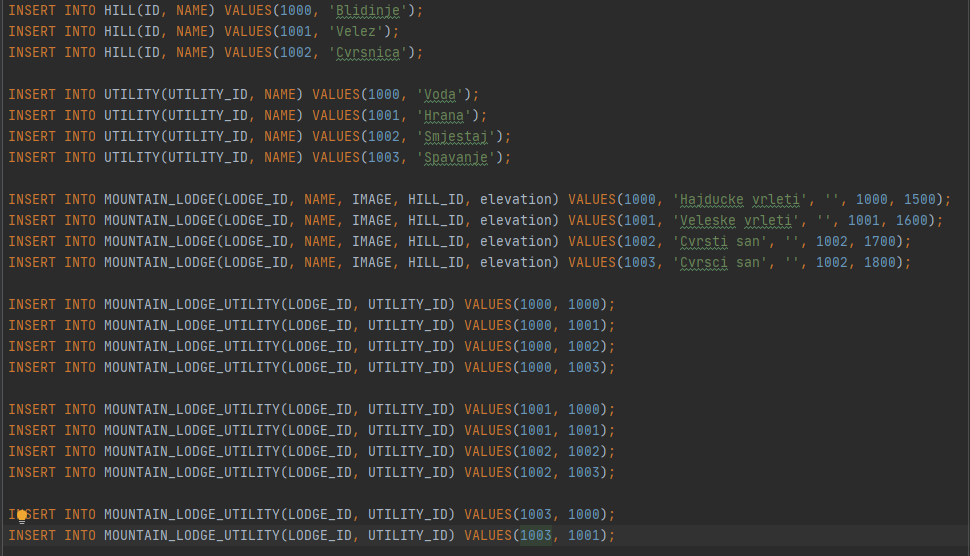
\includegraphics[scale=0.6, height=75mm, width=150mm]{slike/servis-sql.png} %veličina slike u odnosu na originalnu datoteku i pozicija slike
						\centering
						\caption{SQL skripta za testiranje servisnog sloja}
						\label{fig:SQL skripta}
					\end{figure}
					
					\eject 
					 
					
					\textbf{\textit{Ispitni slučaj 8: Pretraga planinarskih domova prema nazivu.}}\\
					Pretražujemo sve planinarske domove koji sadržavaju slovo "v", a infrastrukturne pogodnosti su voda i hrana, predstavljene svojim identifikatorima 1000 odnosno 1001.
					Očekivano ponašanje je povratak 3 planinarska doma.\\
					
					
					\begin{lstlisting}
						@Test
						public void Given_ValidRequestWithUtilities_When_SearchMountainLodgesBySearchCriteria_
						Should_ReturnResultsFromDb(){
							
							MountainLodgeSearchRequest request = new MountainLodgeSearchRequest();
							
							request.setSearchText("v");
							request.setUtilities(List.of(1000L, 1001L));
							
							List<MountainLodge> response = mountainLodgeQueryService.findAllMountainLodgeBySearchCriteria(request);
							
							Assert.assertEquals(3, response.size());
							Assert.assertEquals("Hajducke vrleti", response.get(0).getName());
							Assert.assertEquals("Veleske vrleti", response.get(1).getName());
							Assert.assertEquals("Cvrsci san", response.get(2).getName());
							
							Assert.assertEquals(Long.valueOf(1000), response.get(0).getId());
							Assert.assertEquals(Long.valueOf(1001), response.get(1).getId());
							Assert.assertEquals(Long.valueOf(1003), response.get(2).getId());
						}
					\end{lstlisting}
				
				\textbf{\textit{Ispitni slučaj 9: Pretraga planinarskih domova, sva polja sadržavaju dozvoljene vrijednosti.}}\\
				Očekivani rezultat ovog testa je povratak liste planinarskih domova, čije ime sadržava riječ "vrleti", a nalaze se na planini "Blidinje", identifikatora \textit{1000}.\\
				
							
							\begin{lstlisting}
								@Test
								public void Given_ValidRequest_When_SearchMountainLodgesBySearchCriteria
								_Should_ReturnResultsFromDb(){
									
									MountainLodgeSearchRequest request = new MountainLodgeSearchRequest();
									request.setHillId(1000L);
									request.setSearchText("vrleti");
									request.setUtilities(Collections.emptyList());
									
									List<MountainLodge> response = mountainLodgeQueryService.findAllMountainLodgeBySearchCriteria(request);
									
									Assert.assertEquals(1, response.size());
									Assert.assertEquals("Hajducke vrleti", response.get(0).getName());
									Assert.assertEquals(Long.valueOf(1000), response.get(0).getId());
									Assert.assertEquals(4, response.get(0).getUtilities().size());
									
								}
							\end{lstlisting}
						
						\textbf{\textit{Ispitni slučaj 10: Pretraga planinarskih domova, sva polja sadržavaju dozvoljene vrijednosti, nema rezultata.}}\\
						Očekivani rezultat ovog testa je povratak prazne liste domova, jer dom koji zadovoljava parametre ne postoji u bazi podataka. Parametar koji nije zadovoljen je naziv planinarskog doma "Planinarski dom graficar".\\
						
						\begin{lstlisting}
							@Test
							public void Given_ValidRequestNoMatchingLodgeName_When_SearchMountainLodgesBySearchCriteria_
							Should_ReturnEmptyList(){
								
								MountainLodgeSearchRequest request = new MountainLodgeSearchRequest();
								request.setSearchText("Planinarski dom graficar");
								request.setUtilities(List.of(1000L, 1001L));
								
								List<MountainLodge> response = mountainLodgeQueryService
								.findAllMountainLodgeBySearchCriteria(request);
								Assert.assertEquals(0, response.size());
							}
						\end{lstlisting}
					
					\textbf{\textit{Ispitni slučaj 11: Pretraga planinarskih domova, tekst pretrage velikim slovima.}}\\
					Očekivani rezultat ovog testa je povratak liste koja sadrži jedan dom naziva "Hajducke vrleti".\\
							
				
				\begin{lstlisting}
					@Test
					public void Given_ValidRequestUppercase_When_SearchMountainLodgesBySearchCriteria
					_Should_ReturnOneResult(){
						
						MountainLodgeSearchRequest request = new MountainLodgeSearchRequest();
						request.setSearchText("HAJDUCKE vRlEti");
						
						List<MountainLodge> response = mountainLodgeQueryService.findAllMountainLodgeBySearchCriteria(request);
						Assert.assertEquals(1, response.size());
						Assert.assertEquals("Hajducke vrleti", response.get(0).getName());
					}
				\end{lstlisting}
				
				\subsubsection{Prikaz rezultata testova}
				
				\begin{figure}[H]
					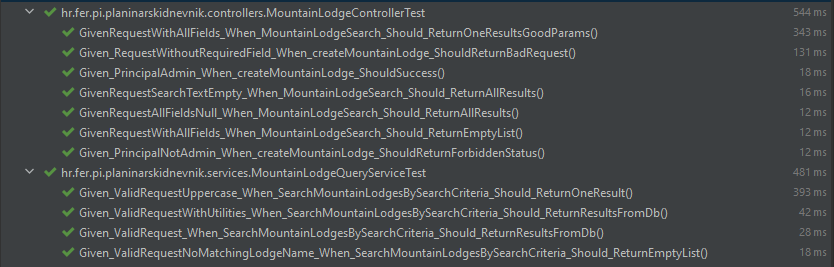
\includegraphics[scale=0.6, height=50mm, width=150mm]{slike/junit.png} %veličina slike u odnosu na originalnu datoteku i pozicija slike
					\centering
					\caption{Rezultati JUnit testova}
					\label{fig:junit testovi}
				\end{figure}
				
				\eject 
			
			
			\subsection{Ispitivanje sustava}
			
			  Ispitivanje smo proveli koristeći Selenium WebDriver unutar JUnit testova. Cilj ispitivanje bio je provjera nekih glavnih funkcionalnosti sustava i pronalazak pogrešaka. WebDriver potrebno je instalirati lokalno na računalo i prilikom pokretanja postaviti putanju koja se nalazi u varijablama okruženja sustava. Prilikom testiranja aplikacija se pokretala na lokalnom računalu zato što je Heroku servis na kojemu je aplikacija puštena u pogon dosta sporiji, pa bi testovi trajali nešto dulje vremena.
			  Slika testova koji su se uspješno izvršili i na aplikaciji puštenoj u pogon na servisu Heroku će biti priložena.\\
	
		
		 	\textbf{\textit{Ispitni slučaj 1: Prijava planinara u sustav s ispravnim/neispravnim podacima}}
		 	
		 	\begin{lstlisting}
		 	public void testLoginBadAndGoodCreds() throws InterruptedException {
		 		//Driver setup...
		 		System.setProperty("webdriver.chrome.driver", "/path...");
		 		WebDriver driver = new ChromeDriver(); 
		 		driver.manage().timeouts().implicitlyWait(Duration.of(20, ChronoUnit.SECONDS));
		 		
		 		driver.get("http://localhost:3000/home");
		 		WebElement loginButton = driver.findElement(By.id("log-button"));
		 		loginButton.click();
		 		String loginUrl = driver.getCurrentUrl();
		 		assertTrue(loginUrl.contains("/login"));
		 		WebElement Emailelement = driver.findElement(By.id("email"));        
		 		Emailelement.sendKeys("luka.ravenscak");   
		 		WebElement passElement = driver.findElement(By.id("password"));
		 		passElement.sendKeys("password");
		 		driver.findElement(By.className("submitButton")).click();
		 		WebElement element = driver.findElement(By.className("errorText"));
		 		assertEquals("Neispravan oblik mail-a.", element.getText());
		 		Emailelement.clear();
		 		Emailelement.sendKeys("luka.ravenscak@fer.hr");
		 		passElement.clear();
		 		passElement.sendKeys("mypassword");
		 		driver.findElement(By.className("submitButton")).click();
		 		element = driver.findElement(By.id("error-span"));
		 		assertEquals("Neispravan e-mail ili lozinka.", element.getText());
		 		passElement.clear();
		 		passElement.sendKeys("password");
		 		driver.findElement(By.className("submitButton")).click();
		 		Thread.sleep(1000);
		 		assertTrue(driver.getCurrentUrl().contains("/mountaineering-community"));
		 		
		 		driver.quit();
		 	}
		 	\end{lstlisting}
	 	
	 	 U 1. ispitnom slučaju ispitana je funkcionalnost prijave u sustav. Prvo se dohvati početna stranica aplikacije te se odabire opcija "Prijavi se" koja se nalazi na zaglavlju stranice. Zatim se unese neispravni oblik email-a, na što aplikacija vraća obavijest "Neispravan oblik mail-a.", nakon toga se unose valjani email i neispravna lozinka, aplikacija reagira tako da vrati obavijest "Neispravan e-mail ili lozinka.". Na kraju se unesu ispravni podaci za prijavu i aplikacija reagira uspješnom prijavnom korisnika u sustav i odvede korisnika na stranicu vlastite planinarske zajednice.\newline
	 	 
	 		\textbf{\textit{Ispitni slučaj 2: Planinar pretražuje ostale korisnike}}
	 	
	 	\begin{lstlisting}
	 		public void testSearchAdminOnAllUserSearchPage() throws InterruptedException {
	 			
	 			//Driver setup
	 			driver.get("http://localhost:3000/login");
	 			
	 			WebElement element = driver.findElement(By.id("email"));        
	 			element.sendKeys("luka.ravenscak@fer.hr");
	 			element = driver.findElement(By.id("password"));
	 			element.sendKeys("password");
	 			driver.findElement(By.className("submitButton")).click();
	 			Thread.sleep(2000);
	 			assertTrue(driver.getCurrentUrl().contains("/mountaineering-community"));
	 			
	 			WebElement searchAllButton = driver.findElement(By.className("search-all-button"));
	 			searchAllButton.click(); 
	 			
	 			assertTrue(driver.getCurrentUrl().contains("/users/search"));    
	 			element = driver.findElement(By.name("searchText"));        
	 			element.sendKeys("admin");
	 			driver.findElement(By.name("searchText")).click();
	 			driver.findElement(By.className("all-user-photo")).click();
	 			Thread.sleep(2000);	    
	 			assertTrue(driver.getCurrentUrl().contains("/profile"));
	 			
	 			assertEquals("admin", driver.findElement(By.id("name-profile")).getAttribute("value"));
	 			driver.quit();
	 		}
	 	\end{lstlisting}
 	
	 	U 2. ispitnom slučaju ispitana je funkcionalnost pretrage svih korisnika od strane planinara. Prvo se provede prijava planinara u sustav, zatim prijavljeni korisnik odabire opciju "Pretraži sve planinare" te ga aplikacija preusmjeri na stranicu za pretragu svih korisnika. Korisnik u prostor za unos teksta za pretragu upiše "admin" i odabire opciju pretrage, aplikacija u rezultatima pretrage vrati traženog korisnika. Nakon toga korisnik odabere adminovu sličicu profila i aplikacija mu prikaže adminov profil. Testiranje je provedeno na način da se pretražuje profil admina, koji unutar aplikacije uvijek postoji.\newline
	 	
 		\textbf{\textit{Ispitni slučaj 3: Pretraga i arhiviranje posjećenog planinarskog doma}}
 		
 		\begin{lstlisting}
 			public void testMountainLodgeSearchArchiveAndBadgeAdd() throws InterruptedException {
 			//Driver setup
 			
 			driver.get("http://localhost:3000");
 			driver.findElement(By.className("domovi")).click();
 			assertTrue(driver.getCurrentUrl().contains("/mountain-lodge/search"));
 			driver.findElement(By.className("input-search")).sendKeys("Planinarski dom Glavica");	    
 			driver.findElement(By.className("search-button")).click();
 			assertEquals("Planinarski dom Glavica", driver.findElement(By.className("mountain-lodge-name")).getText());
 			assertThrows(NoSuchElementException.class, new ThrowingRunnable() {
 				public void run() throws Throwable {
 					driver.findElement(By.className("archive-button-lodge"));
 				}
 			});
 			
 			WebElement loginButton = driver.findElement(By.id("log-button"));
 			loginButton.click();
 			String loginUrl = driver.getCurrentUrl();
 			assertTrue(loginUrl.contains("/login"));
 			WebElement Emailelement = driver.findElement(By.id("email"));        
 			Emailelement.sendKeys("luka.ravenscak@fer.hr");   
 			WebElement passElement = driver.findElement(By.id("password"));
 			passElement.sendKeys("password");
 			driver.findElement(By.className("submitButton")).click();
 			Thread.sleep(2000);
 			assertTrue(driver.getCurrentUrl().contains("/mountaineering-community"));
 			driver.findElement(By.className("logo-image")).click();
 			
 			driver.findElement(By.className("domovi")).click();
 			assertTrue(driver.getCurrentUrl().contains("/mountain-lodge/search"));
 			driver.findElement(By.className("input-search")).sendKeys("Planinarski dom Glavica");	    
 			driver.findElement(By.className("search-button")).click();
 			assertEquals("Planinarski dom Glavica", driver.findElement(By.className("mountain-lodge-name")).getText());
 			
 			WebElement archiveButton = driver.findElement(By.className("archive-button-lodge"));
 			assertEquals("ARHIVIRAJ",driver.findElement(By.className("MuiButton-label"))
 			.getText());
 			archiveButton.click();
 			Thread.sleep(3000);
 			assertEquals("ARHIVIRANO",driver.findElement(By.className("MuiButton-label"))
 			.getText());
 			
 			driver.findElement(By.className("profil-image")).click();
 			driver.findElement(By.id("my-profile")).click();
 			String badgeDesc = driver.findElement(By.className("badge-image")).getAttribute("title");
 			assertEquals("Imam barem 1 posjecen planinarski dom!", badgeDesc);
 			
 			driver.quit();
 		}
 		\end{lstlisting}
 	
 		U 3. ispitnom slučaju ispitana je funkcionalnost pretraživanja i arhiviranja planinarskog doma, te je testirano da pristup arhiviranju imaju samo prijavljeni korisnici. Neprijavljen korisnik odabire opciju "Pretraga planinarskih domova", u prostor za unos teksta upisuje "Planinarski dom Glavica". Taj dom postoji u bazi podataka i aplikacija mu kao rezultat pretrage prikaže traženi planinarski dom. Zatim se testira da aplikacija neprijavljenom korisniku ne nudi mogućnost arhiviranja doma. Nakon što je taj dio testa aplikacija zadovoljen, test se nastavlja i korisnik se prijavi u sustav kao planinar te ponavlja istu radnju. Ovaj put aplikacija mu prikazuje traženi dom, ali korisnik ima mogućnost arhiviranja doma. Korisnik odabire opciju "Arhiviraj", aplikacija na tu akciju mijenja opis uz navedeni dom u "Arhivirano", te odabrani dom sprema u popis posjećenih domova planinara koji je odabrao opciju "Arhiviraj". Korisnik odabire opciju "Moj profil", aplikacija mu prikaže profil na kojem se može vidjeti priznanje (bedž) kojeg je dobio posjetom jednog planinarskog doma, uz opis postignuća "Imam barem 1 posjećen planinarski dom!"\newline
 		
 		 	\textbf{\textit{Ispitni slučaj 4: Slanje zahtjeva za prijateljstvo i primitak obavijesti o prihvaćenom zahtjevu}}
 		
 		\begin{lstlisting}
 			public void testAddFriendAndFriendRequestApproveOrDeclineAndFriendNotification() throws InterruptedException {
 				//Driver setup
 				
 				driver.get("http://localhost:3000/login");      
 				driver.findElement(By.id("email")).sendKeys("luka.ravenscak@fer.hr");   
 				driver.findElement(By.id("password")).sendKeys("password");
 				driver.findElement(By.className("submitButton")).click();
 				Thread.sleep(2000);
 				
 				WebElement searchAllButton = driver.findElement(By.className("search-all-button"));
 				searchAllButton.click(); 
 				assertTrue(driver.getCurrentUrl().contains("/users/search"));
 				WebElement element = driver.findElement(By.name("searchText"));        
 				element.sendKeys("admin");
 				driver.findElement(By.name("searchText")).click();
 				driver.findElement(By.className("all-user-photo")).click();
 				Thread.sleep(2000);	    
 				assertTrue(driver.getCurrentUrl().contains("/profile"));
 				
 				driver.findElement(By.className("button-profile")).click();
 				assertTrue(driver.findElement(By.className("button-profile-fr"))
 				.getText().contains("Zahtjev poslan"));
 				driver.findElement(By.className("profil-image")).click();
 				driver.findElement(By.id("logout-b")).click();
 				Thread.sleep(2000);
 				driver.findElement(By.id("log-button")).click();
 				driver.findElement(By.id("email")).sendKeys("admin@fer.hr");   
 				driver.findElement(By.id("password")).sendKeys("password");
 				driver.findElement(By.className("submitButton")).click();
 				Thread.sleep(2000);
 				driver.findElement(By.className("profil-image")).click();
 				driver.findElement(By.id("fr-requests")).click();
 				assertEquals("Luka Ravenscak", driver.findElement(By.className("user-name")).getText());
 				driver.findElement(By.className("submitButtonaccept")).click();
 				
 				driver.findElement(By.className("profil-image")).click();
 				driver.findElement(By.id("logout-b")).click();
 				Thread.sleep(2000);
 				driver.findElement(By.id("log-button")).click();
 				driver.findElement(By.id("email")).sendKeys("luka.ravenscak@fer.hr");   
 				driver.findElement(By.id("password")).sendKeys("password");
 				driver.findElement(By.className("submitButton")).click();
 				Thread.sleep(2000);
 				driver.findElement(By.className("profil-image")).click();
 				driver.findElement(By.id("fr-notifications")).click();
 				assertTrue(driver.findElement(By.className("user-name-span"))
 				.getText().contains("Postali ste prijatelj s"));
 				assertTrue(driver.findElement(By.className("user-name"))
 				.getText().contains("admin"));
 				driver.quit();
 			}
 		\end{lstlisting}
 	
 		U 4. ispitnom slučaju ispitana je funkcionalnost slanja zahtjeva za prijateljstvo i primanje obavijesti o prihvaćenom zahtjevu. Prvo se korisnik prijavi kao "luka.ravenscak@fer.hr" te provede radnje kao u testu 2. Dolaskom na adminov profil odabere opciju "Dodaj prijatelja". Aplikacija promijeni status gumba u "Zahtjev poslan" te proslijedi zahtjev za prijateljstvo adminu. Zatim se korisnik odjavi, te odlazimo na profil admina, nakon čega korisnik provjeri zahtjeve za prijateljstvo i prihvati zahtjev korisnika "luka.ravenscak@fer.hr".
 		Nakon što je admin uspješno prihvatio zahtjev korisnik se odjavi i prijavi ponovno kao "luka.ravenscak@fer.hr". Nakon toga aplikacija će korisniku "luka.ravenscak@fer.hr" prikazati novu obavijest o prihvaćenom zahtjevu za prijateljstvo od strane admina. 
 		
		
		\begin{figure}[H]
			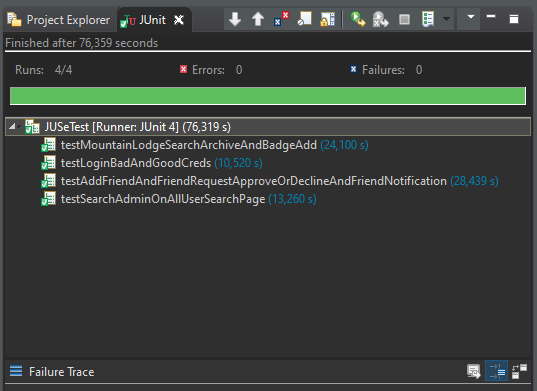
\includegraphics[scale=0.6, height=65mm, width=100mm]{slike/test_results.png} %veličina slike u odnosu na originalnu datoteku i pozicija slike
			\centering
			\caption{Uspješno izvršeni Selenium testovi - lokalno računalo}
			\label{fig:test_results}
		\end{figure}
		
			\eject 
		
		
		\section{Dijagram razmještaja}
			
			Dijagrami razmještaja opisuju topologiju fizikalnih uređaja i radnih okruženja koja se koriste u implementaciji sustava. Na korisničkom računalu se nalazi web poslužitelj kao pristupna točka aplikaciji. Na samom poslužitelju imamo našu PostgreSQL bazu podataka i backend koji služi za razmjenu HTTP zahtjeva s korisnikom i obrađivanje transakcija s bazom podataka. Sustav je baziran na arhitekturi "klijent - poslužitelj".
			 
			\begin{figure}[H]
				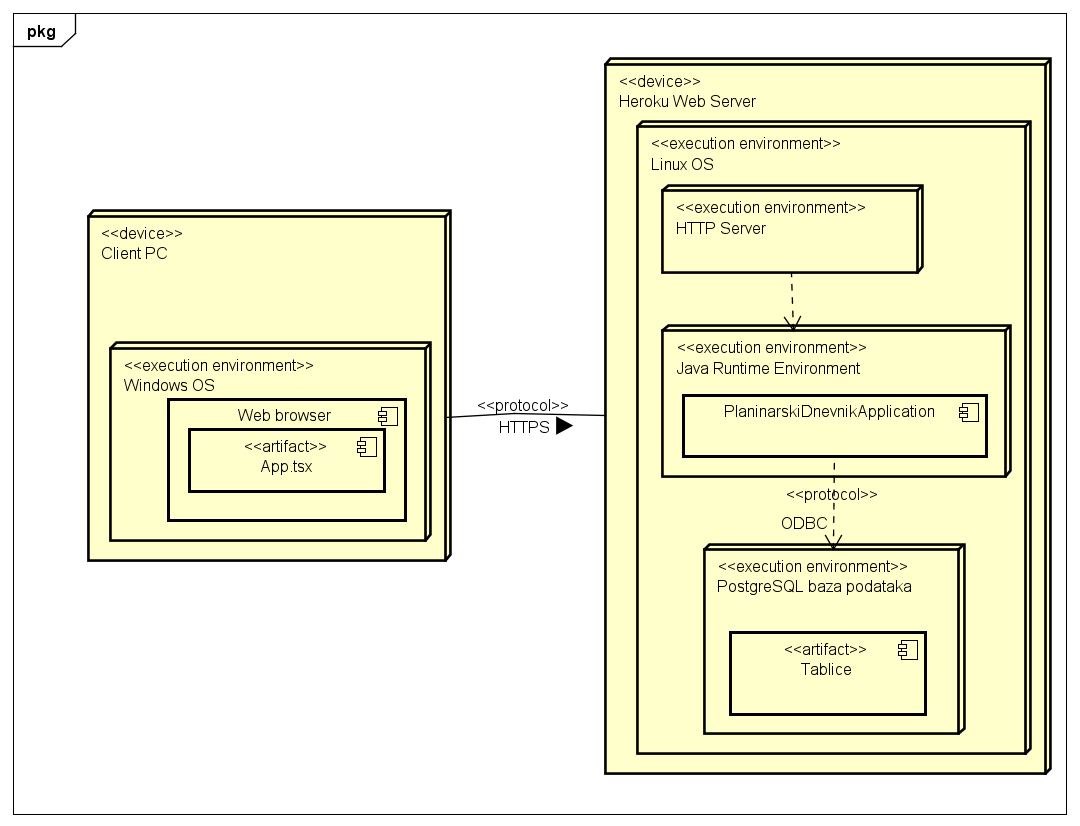
\includegraphics[width=160mm, height=155mm]{dijagrami/deployment diagram.png} %veličina slike u odnosu na originalnu datoteku i pozicija slike
				\centering
				\caption{Dijagram razmještaja}
				\label{fig:dijagramdeployment}
			\end{figure}
			\eject 
		
		\section{Upute za puštanje u pogon}
		
			U ovom poglavlju će biti opisano puštanje aplikacije u pogon, odnosno jedan od načina da se od izvornog koda dođe do funkcionalne aplikacije koja odgovara na upite.
			Aplikacija je u pogon puštena na servis Heroku\footnote{https://www.heroku.com/home} (platforma kao usluga). Prije početka, potrebno je napraviti korisnički račun na toj platformi, pritiskom na gumb \textbf{Sign up for free}, a nakon toga i prijaviti\footnote{https://id.heroku.com/login} na platformu. Nakon prijave otvara se ekran koji prikazuje popis Vaših aplikacija te mogućnost stvaranja nove aplikacije, kao na slici. Ako ste se prvi put registrirali, ovaj popis će biti prazan.
			\begin{figure}[H]
				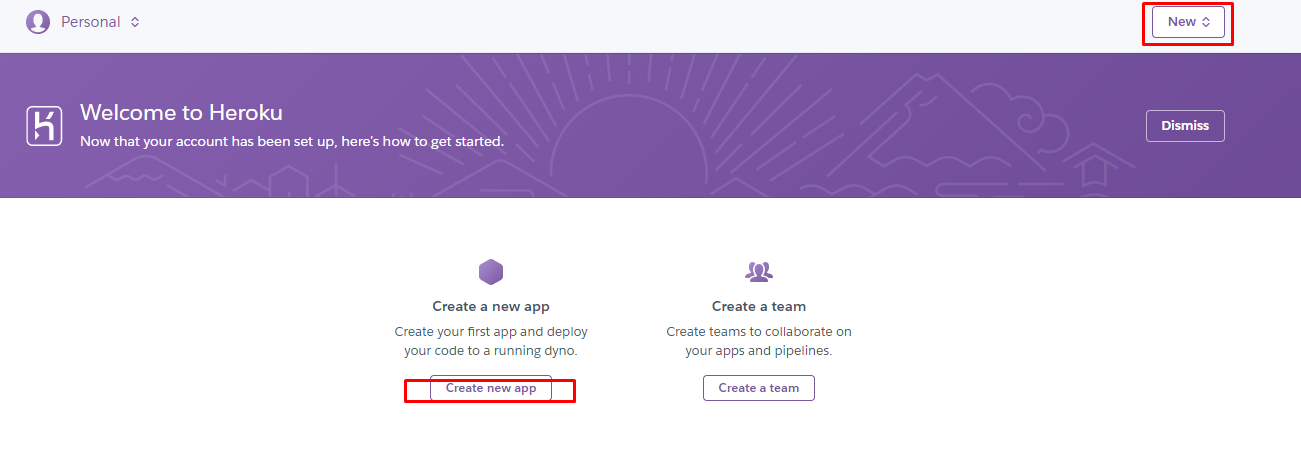
\includegraphics[width=170mm, height=70mm]{slike/heroku-dash.png} %veličina slike u odnosu na originalnu datoteku i pozicija slike
				\centering
				\caption{Heroku dashboard}
				\label{fig:dijagramdeployment}
			\end{figure}
			\eject 
			
			Pritiskom na gumb za stvaranje nove aplikacije, otvara se prozor kao na slici, gdje unosite željeni naziv aplikacije, u našem slučaju \textit{deploy-demo-frontend}.
			
			\begin{figure}[H]
				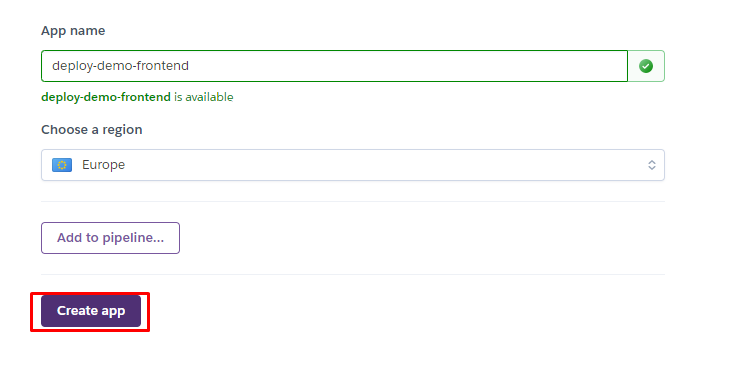
\includegraphics[width=120mm, height=80mm]{slike/heroku-create-fr.png} %veličina slike u odnosu na originalnu datoteku i pozicija slike
				\centering
				\caption{Stvaranje frontenda - Heroku}
				\label{fig:dijagramdeployment}
			\end{figure}
			\eject 
			
			Nakon toga se otvara upravljač za Vašu aplikaciju, odaberite \textbf{Settings} te nakon toga gumb \textbf{Add buildpack}, kao na slici.
			
			\begin{figure}[H]
				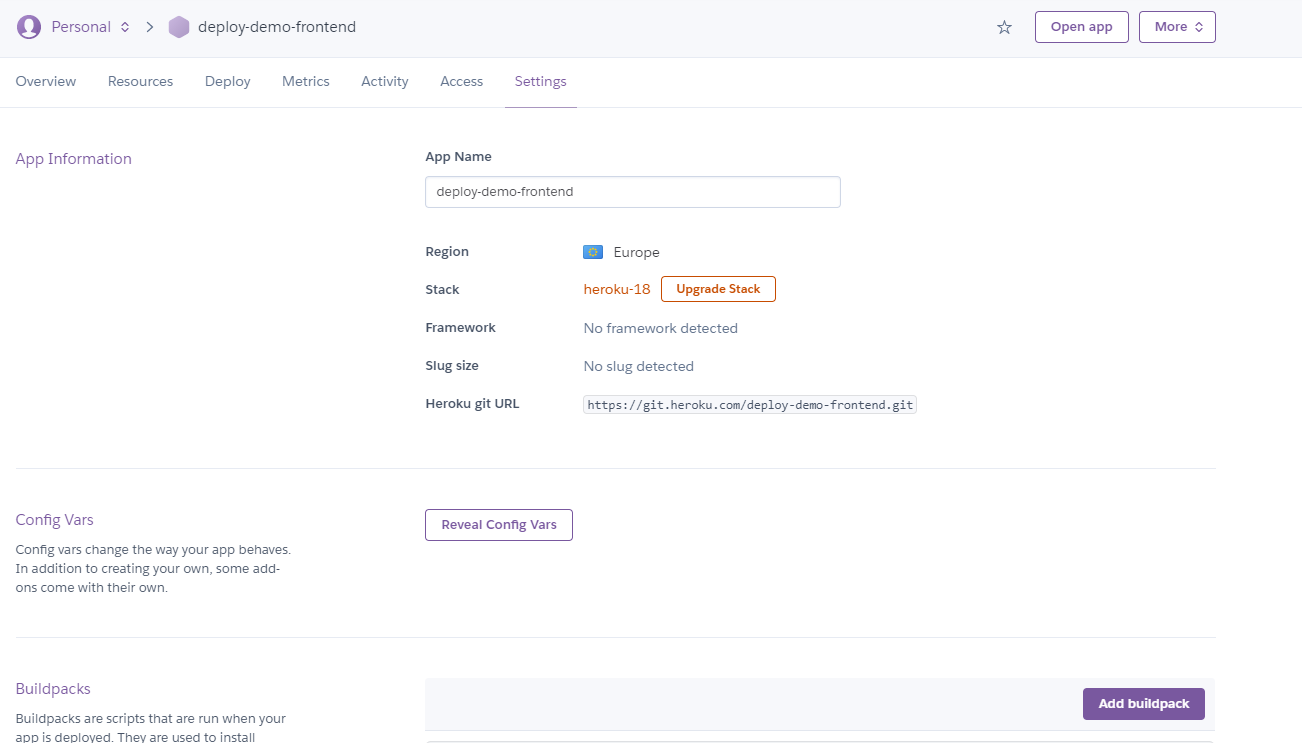
\includegraphics[width=160mm, height=140mm]{slike/heroku-settings.png} %veličina slike u odnosu na originalnu datoteku i pozicija slike
				\centering
				\caption{Dodavanje buildpacka}
				\label{fig:dijagramdeployment}
			\end{figure}
			\eject 
			Nakon otvaranja novog prozora, upište sljedeći URL: \textit{https://github.com/mars/create-react-app-buildpack.git}, kao na slici.
			\begin{figure}[H]
				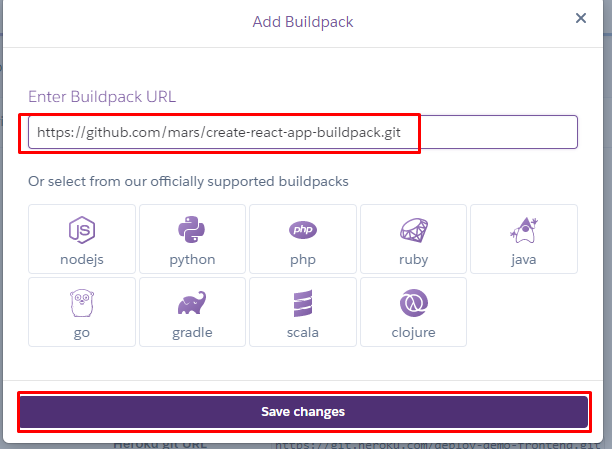
\includegraphics[width=130mm, height=80mm]{slike/heroku-buildp.png} %veličina slike u odnosu na originalnu datoteku i pozicija slike
				\centering
				\caption{Dodavanje buildpacka}
				\label{fig:dijagramdeployment}
			\end{figure}
			
			Na istom mjestu možete pronaći i domenu Vaše aplikacije, ona će uvijek biti u obliku \textbf{https://APP-NAME.herokuapp.com/}, gdje je APP-NAME Vaš odabrani naziv aplikacije. U našem slučaju to bi bilo: \textbf{https://deploy-demo-frontend.herokuapp.com/}.
			Na analogan način treba postupiti i s dodavanjem poslužiteljskog dijela aplikacije, samo ovoga puta nakon stvaranja aplikacije \textbf{nije potrebno dodavati buildpack} zato što je poslužiteljski dio aplikacije pisan u Javi, s \textit{Gradle-om} kao upravljačem.
			
			Za dodavanje \textit{PostgreSQL} baze podataka na backendu, nakon stvaranja aplikacije pratite niže navedene korake. Prilikom odabira za koju aplikaciju stvarate bazu podataka, odaberite poslužiteljsku stranu, u našem slučaju \textit{deploy-demo-backend}.
			
			\begin{figure}[H]
				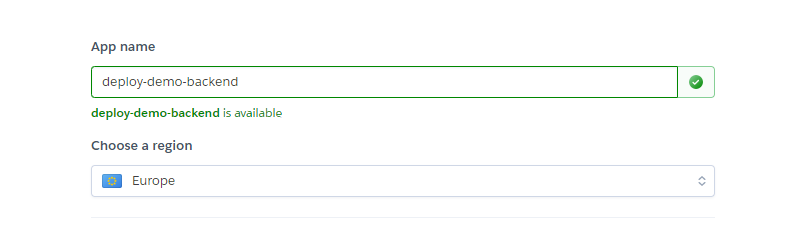
\includegraphics[width=110mm, height=60mm]{slike/heroku-create-b.png} %veličina slike u odnosu na originalnu datoteku i pozicija slike
				\centering
				\caption{Dodavanje backenda}
				\label{fig:dijagramdeployment}
			\end{figure}
			\begin{figure}[H]
				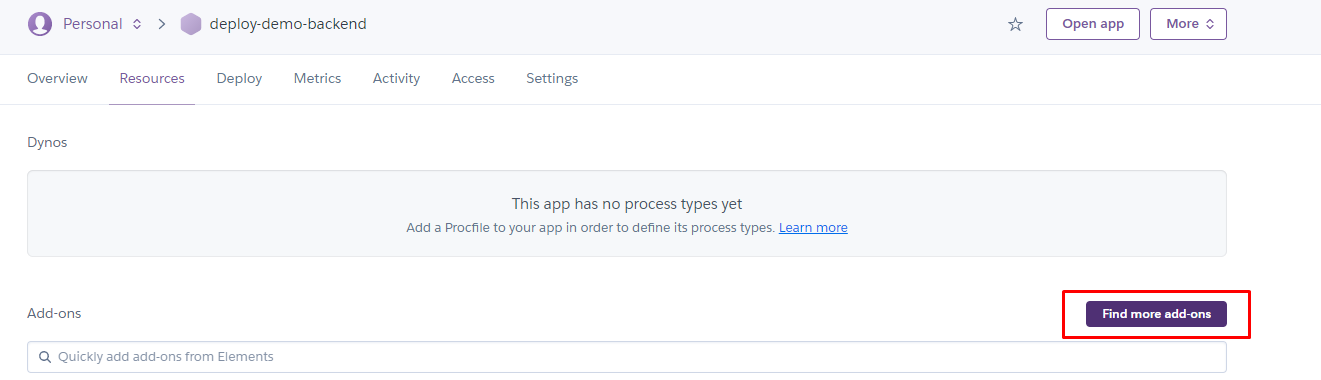
\includegraphics[width=150mm, height=70mm]{slike/heroku-adddb.png} %veličina slike u odnosu na originalnu datoteku i pozicija slike
				\centering
				\caption{Dodavanje baze podataka prvi korak}
				\label{fig:dijagramdeployment}
			\end{figure}
			\begin{figure}[H]
				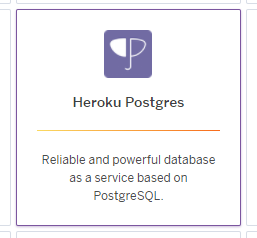
\includegraphics[width=50mm, height=50mm]{slike/heroku-pgaddon.png} %veličina slike u odnosu na originalnu datoteku i pozicija slike
				\centering
				\caption{Dodavanje baze podataka drugi korak}
				\label{fig:dijagramdeployment}
			\end{figure}
			\begin{figure}[H]
				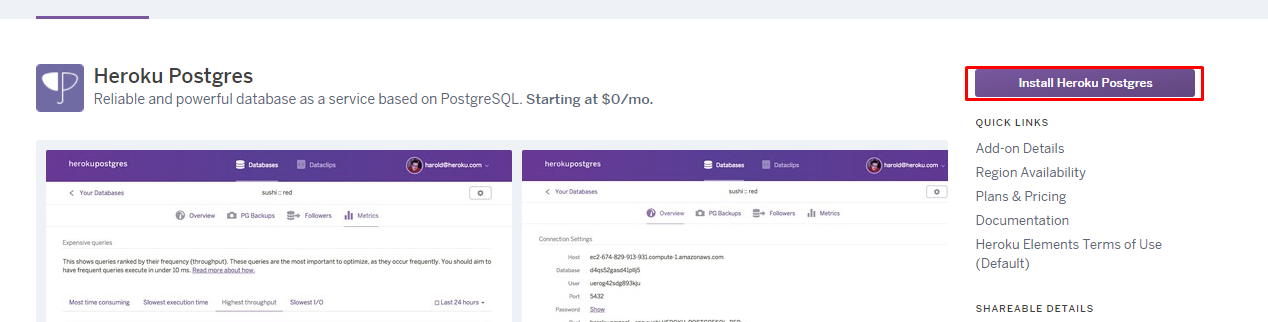
\includegraphics[width=130mm, height=60mm]{slike/heroku-insaddon.png} %veličina slike u odnosu na originalnu datoteku i pozicija slike
				\centering
				\caption{Dodavanje baze podataka treći korak}
				\label{fig:dijagramdeployment}
			\end{figure}
			\begin{figure}[H]
				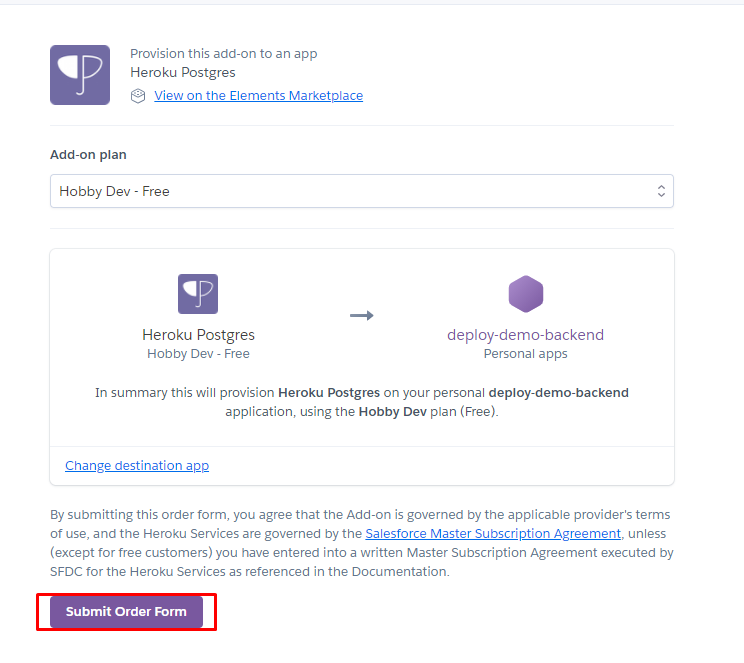
\includegraphics[width=130mm, height=60mm]{slike/heroku-submit.png} %veličina slike u odnosu na originalnu datoteku i pozicija slike
				\centering
				\caption{Dodavanje baze podataka četvrti korak}
				\label{fig:dijagramdeployment}
			\end{figure}
			
			Sada je sve spremno za postavljanje našeg izvornog koda na udaljeni poslužitelj koji pruža \textit{Heroku}.
			
			Nakon stvaranja aplikacija na Heroku i uspostavljanja baze, sa URL-a \footnote{https://gitlab.com/Pi-FER/RuntimeTerror/-/tree/final-deploy/IzvorniKod} potrebno je preuzeti naš Izvorni kod, preporučljivo kao ZIP arhivu zbog monorepozitorija, te ju raspakirati na lokalnom računalu. Nakon toga potrebno je preuzeti \textit{HerokuCLI}\footnote{https://devcenter.heroku.com/articles/heroku-cli}.
			Nakon što ste preuzeli izvorni kod, pozicionirajte se u direktorij \textit{IzvorniKod} u Vašem terminalu.
			Nakon toga unesite naredbu 
			
			\begin{lstlisting}[language=bash]
				heroku login
			\end{lstlisting}
			 te se prijavite na Vaš Heroku korisnički račun.
			\begin{figure}[H]
				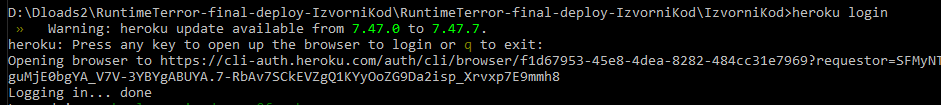
\includegraphics[width=160mm]{slike/h-login.png} %veličina slike u odnosu na originalnu datoteku i pozicija slike
				\centering
				\caption{Dodavanje baze podataka četvrti korak}
				\label{fig:dijagramdeployment}
			\end{figure}
			Nakon toga je potrebno otvoriti: 
			\begin{lstlisting}[language=bash]
				IzvorniKod\frontend\src\Util.ts
			\end{lstlisting}
			te zamijeniti postojeći varijablu \textbf{PROD\_ENV} URL-om Vašeg poslužiteljskog dijela aplikacije. Na slici je prikazan URL u ovom demonstracijskom slučaju.
			\begin{lstlisting}[language=bash]
				const PROD_ENV = "https://deploy-demo-backend.herokuapp.com";
			\end{lstlisting}
		
			Nakon ovoga klijentska strana aplikacije spremna je za puštanje u pogon.	
			Isti postupak ćemo napraviti i na poslužiteljskoj strani, otvorite datoteku:
			\begin{lstlisting}[language=bash]
				IzvorniKod\backend\src\hr\fer\src\main\java\pi\planinarskidnevnik
				\PlaninarskiDnevnikApplication.java
			\end{lstlisting}
			te u dopuštene izvore dodajte URL Vaše klijentske strane aplikacije. U našem slučaju to bi izgledalo ovako:
			
			\begin{lstlisting}[language=java]
				allowedOrigins("https://deploy-demo-frontend.herokuapp.com")
			\end{lstlisting}
			Nakon toga se pozicionirajte u \textit{IzvorniKod} te unesite redom naredbe:
			\begin{lstlisting}[language=bash]
				cd backend
				git init
				heroku git:remote -a deploy-demo-backend
				
				git add .
				git commit -am "initial commit"
				git push heroku master
			\end{lstlisting}
			
			gdje ćete umjesto \textbf{deploy-demo-backend} unijeti ime Vašeg poslužiteljskog dijela aplikacije. Nakon nekoliko minuta će proces unutar naredbenog retka završiti porukom uspjeha te je poslužiteljski dio aplikacije pušten u pogon.
			
			Preostalo je još u pogon pustiti klijentski dio aplikacije. Unesite sljedeće naredbe:
			\begin{lstlisting}[language=bash]
				cd ../frontend
				git init
				heroku git:remote -a deploy-demo-frontend
				
				git add .
				git commit -am "initial commit"
				git push heroku master
			\end{lstlisting}
			gdje ćete umjesto \textbf{deploy-demo-frontend} unijeti ime Vašeg klijentskog dijela aplikacije. Ovaj proces će potrajati nekoliko minuta duže od poslužiteljskog dijela aplikacije. Naravno, pretpostavka je da imate instaliran \textit{Git}\footnote{https://git-scm.com/}.
			Nakon završetka, aplikacija za demonstraciju puštanja u pogon je dostupna na URL-u.\footnote{https://deploy-demo-frontend.herokuapp.com/home}
			Stvarna aplikacija dostupna je na \textbf{URL-u.}\footnote{https://pdnevnik.herokuapp.com/}.
			\begin{figure}[H]
				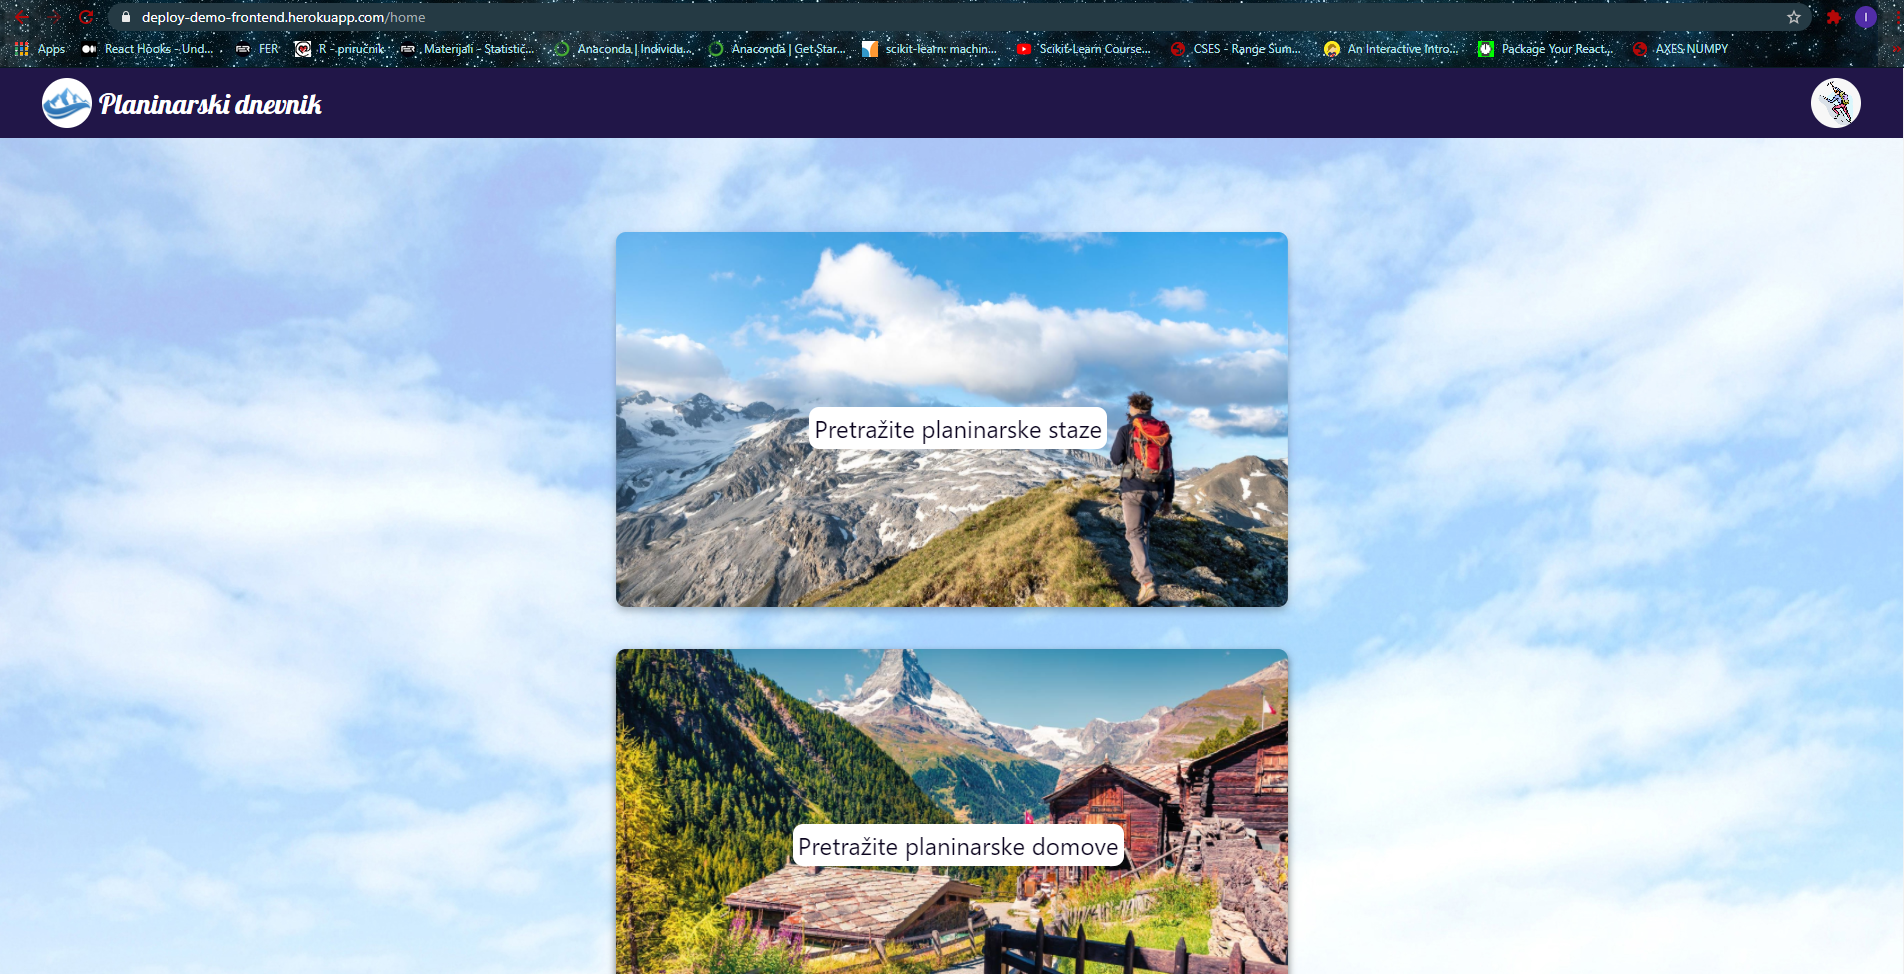
\includegraphics[width=160mm, height=130mm]{slike/app-end.png} %veličina slike u odnosu na originalnu datoteku i pozicija slike
				\centering
				\caption{Aplikacija puštena u pogon}
				\label{fig:dijagramdeployment}
			\end{figure}
			\eject 